\chapter{Wireless Interface} \label{sec:wireless}

Four methods of a wireless connection have been considered: Bluetooth (perhaps with CC2541), WiFi with ESP8266, a 868\,MHz long range link with SX1276, and a 2.4\,GHz link with nRF24L01+. Bluetooth was dismissed early for its complexity, and ESP8266 for its high consumption in continuous reception mode, although both solutions might be viable for certain applications and with more development time.

The Semtech SX1276~\cite{semtech-manual} and Nordic Semiconductor nRF24L01+ ~\cite{nrf-manual} transceivers have both been tested using the first GEX prototype, proving its usefulness as a hardware development tool, and it has been confirmed they could fulfill the requirements of our application.

\begin{figure}[h]
	\centering
	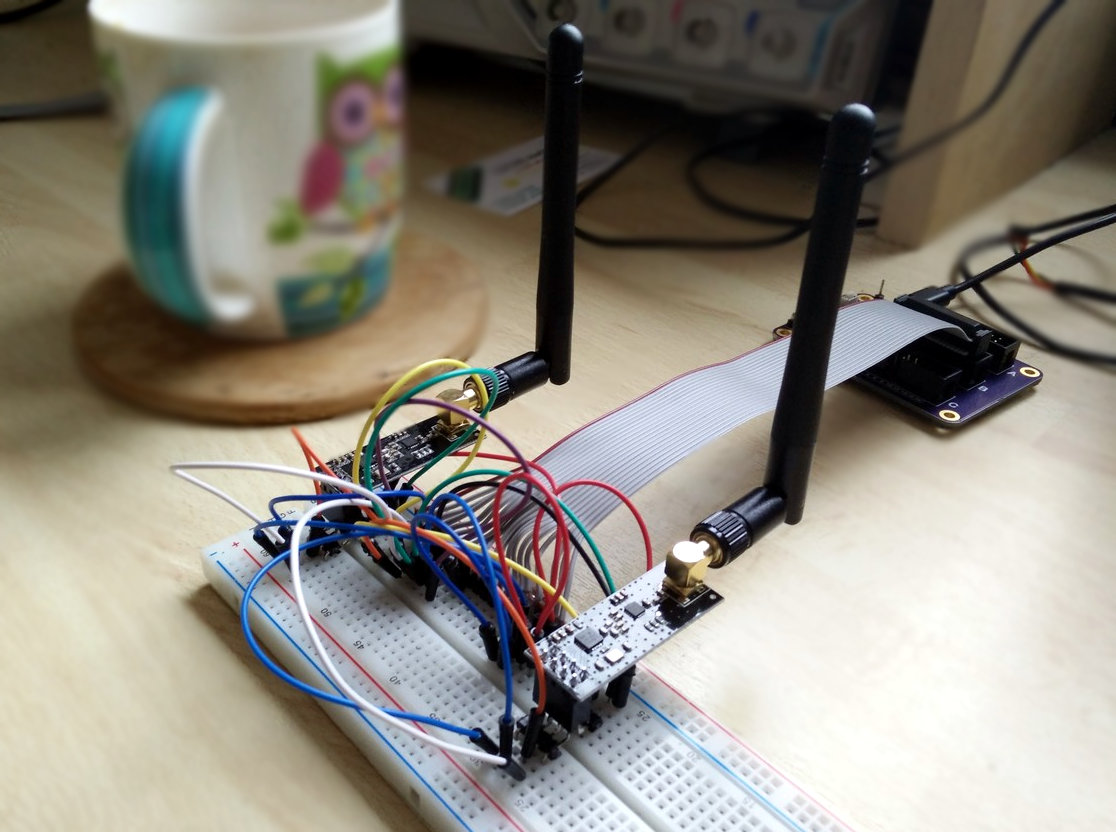
\includegraphics[width=.7\textwidth]{img/nrf-testing.jpg}
	\caption{Test setup with a GEX prototype controlling two nRF24L01+ modules}
\end{figure}

\section{Modulations Overview}

A brief overview of the different signal modulation techniques is presented here to aid the reader with understanding of \cref{fig:nrf-sx-comparison} and the rest of the chapter.

\subsection{On-Off Keying (OOK)}

In \gls{OOK}, the carrier generator is switched on and off to transmit ones and zeros.

\subsection{Frequency Shift Keying (FSK)}

\Gls{FSK} uses a change of the carrier frequency to transmit data. The simplest form of \gls{FSK} is \gls{BFSK}, which uses a pair of alternating frequencies to transmit ones and zeros.

\subsection{Gaussian Frequency Shift Keying (GFSK)}

\Gls{GFSK} is an improvement over basic \gls{FSK} which does not switch between the different frequencies instantaneously, but uses a Gaussian filter to make the changes less abrupt, which reduces the side-band interference otherwise generated by the sharp edges. This scheme can be imagined as sending the binary waveform through a Gaussian filter and then modulating a \gls{VCO} with its output, rather than changing the \gls{VCO}'s control voltage discretely. \Gls{GFSK} is used in the Bluetooth standard.

\subsection{Minimum-Shift Keying (MSK)}

\Gls{MSK} is another \gls{FSK}-based modulation scheme. In \gls{MSK}, the frequencies representing different symbols are chosen such that there are no sharp changes in the phase of the output waveform, the modulation is \textit{phase-coherent}. This is another way to reduce side-band interference.

\subsection{Gaussian Minimum-Shift Keying (GMSK)}

\Gls{GMSK} is a variant of \gls{MSK} which uses a Gaussian filter to shape the digital signal before sending it to the oscillator. The principle is similar to \gls{GFSK}, and it is a yet another way to reduce side-band interference and increase spectral efficiency. \gls{GMSK} is used in the \gls{GSM}.

\subsection{LoRa Modulation}

LoRa is a patented proprietary modulation developed by Semtech. It uses a direct sequence frequency hopping spread spectrum modulation and can achieve very long range transmission (over 10\,km is not uncommon). LoRa is available only with transceiver \glspl{IC} produced by Semtech and for this reason it is rather expensive.

\section{Comparing SX1276 and nRF24L01+}

The two transceivers are compared in \cref{fig:nrf-sx-comparison}. It is apparent that each of them has its strengths and weaknesses, which will be discussed below.

\begin{table}[h]
	\centering
	\begin{tabulary}{\textwidth}{lLL}
		\toprule
		\textbf{Parameter} & \textbf{SX1276} & \textbf{nRF24L01+} \\
		\midrule
		\textbf{Connection} & SPI (4 pins) + up to 6 IRQ & SPI (4 pins), CE, IRQ \\
		\textbf{Frequency band} & 868\,MHz or 433\,MHz & 2.4\,GHz \\
		\textbf{Data rate} & up to 300\,kbps & 250--2000\,kbps \\
		\textbf{Modulation} & (G)FSK, (G)MSK, OOK, LoRa & GFSK \\
		%		\textbf{Bandwidth} & 7--500\,kHz per channel & 0.7--2\,MHz per channel \\
		\textbf{Range (est.)} & over 10\,km & up to 1\,km \\
		\textbf{Consumption Rx} & 10.8--12\,mA & 12.6--13.5\,mA \\
		\textbf{Consumption Tx} & 20--120\,mA & 7--11.3\,mA \\
		\textbf{Idle power (max)} & 1\,$\mu$A sleep, 2\,mA stand-by & 0.9\,$\mu$A sleep, 320\,$\mu$A stand-by \\
		\textbf{Max packet size} & 300 bytes & 32 bytes \\
		\textbf{Reset} & NRESET pin & Vdd disconnect \\
		\textbf{Extra} & LoRa FHSS, packet engine & ShockBurst protocol engine \\
		\textbf{Price} & \$7.3 & \$1.6 \\
		\bottomrule
	\end{tabulary}
	\caption[Comparison of the SX1276 and nRF24L01+ wireless transceivers]{\label{fig:nrf-sx-comparison}Comparison of the SX1276 and nRF24L01+ wireless transceivers, using data from their datasheets (price in USD from DigiKey in a 10\,pcs. quantity, recorded on May 6th 2018)}
\end{table}

SX1276 supports additional modulation modes, including a proprietary LoRa scheme with a frequency-hopping spread spectrum modulation that can be received at a distance up to 20\,km in ideal conditions. The long-range capability is reflected in a higher consumption during transmission. However, its consumption in receiver mode is slightly lower than that of the nRF24L01+.

nRF24L01+ provides higher data rates at short distances. Its power consumption is comparable or lower than that of the SX1276. It lacks a dedicated reset pin, but that can be easily worked around using an external transistor to momentarily disconnect its Vdd pin.

Both devices implement some form of a packet engine with error checking; that of the nRF24L01+, called ShockBurst, is more advanced as it implements acknowledgment responses and automatic re-transmission, leading to a potentially more robust communication without an additional overhead on the side of the microcontroller.


\section{Integration of the nRF24L01+ into GEX}

The nRF24L01+ was selected to be integrated into GEX thanks to its inclusion of the ShockBurst engine, higher possible data rates and significantly lower price. The SX1276, nonetheless, remains an interesting option that could be used as an alternative in the future, should the need for a long range communication arise.

A separate device, the \textit{GEX wireless gateway}, was developed to provide the PC connection to a nRF24L01+ module. It is based on the STM32F103 microcontroller in its smallest package (LQFP48), selected for its low cost and good availability.

\todo[inline]{more about the hardware}

\subsection{The Wireless Gateway Protocol}

\begin{wrapfigure}[17]{r}{0.38\textwidth}
	\vspace{-1em}
	\centering
	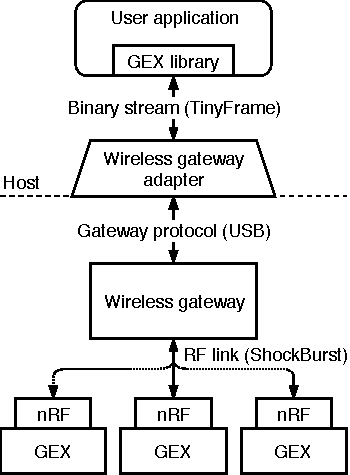
\includegraphics[scale=0.9]{img/rf-gw.pdf}
	\caption{A block diagram of the wireless connection}
\end{wrapfigure}

The gateway presents itself to the host as a \gls{CDCACM} device, much like the GEX modules themselves (here called \textit{nodes}) when connected over \gls{USB}. It implements a simple protocol which encapsulates the binary data sent to or from a connected node. The wrapped GEX protocol, which is described in \cref{sec:tinyframe}, remains unchanged.

The gateway has a 4-byte network ID, a number derived from the \gls{MCU}'s unique ID by calculating its 32-bit \gls{CRC}. The network ID must be entered into all nodes that wish to communicate with the gateway. Additionally, each module is assigned a 1-byte number which serves as its address in the network. The gateway can receive messages from up to 6 nodes.

All messages sent to or from the gateway are a multiple of 64 bytes long, padded with zeros if shorter. The message starts with a control byte determining its type, as summarized in the following table:

{
\tabulinesep=5pt
\begin{longtabu} to \textwidth {P{5em}  X[5] X[4,l]}
	\toprule
	\textbf{First byte} & \textbf{Function} & \textbf{Structure} \\
	\midrule
	\endhead

	\bottomrule
	\endfoot

	`r' (114) &
	\cname{RESTART}
	Restart the gateway, disconnecting all nodes. This is functionally equivalent to re-plugging it to the USB port.
	& \\

	`i' (105) &
	\cname{GET\_NET\_ID}
	Read the unique 4-byte network ID. This command has no side effects and may be used as ``ping'' to verify the USB connection. &
	\begin{cmdresp}
		\cfield{0x01}
		\cfield{u8[4]} network ID
	\end{cmdresp}
	\\

	`n' (110) &
	\cname{ADD\_NODES}
	Configure the gateway to listen for messages from the given nodes.
	Nodes may be removed using the RESTART command.
	&
	\begin{cmdreq}
		\cfield{u8} count
		\cfield{u8[]} node addresses
	\end{cmdreq}
	\\

	`m' (109)&
	\cname{SEND\_MSG}
	Send a binary message to one of the connected nodes. The message may span multiple 64-byte frames; the subsequent frames will contain only the payload bytes, or zero padding at the end of the last one.
	& \begin{cmdreq}
		\cfield{u8} node address
		\cfield{u16} length
		\cfield{u8} checksum (inverted XOR of all payload bytes)
		\cfield{u8[]} payload
	\end{cmdreq} \\

	0x02 &
	\cname{INCOMING\_MSG}
	A message was received from one of the configured nodes. This is an event frame sent by the gateway to the host.
	& \begin{cmdpld}
		\cfield{u8} node address
		\cfield{u8} message length
		\cfield{u8[]} payload
	\end{cmdpld} \\

\end{longtabu}
}

\subsection{Gateway Initialization Procedure}

A host program connecting to a node or nodes through the gateway should follow the following procedure to initialize and configure the gateway:

\begin{enumerate}
	\item Send the `GET\_NET\_ID' command to test if the gateway is connected (and obtain its network ID as a side effect)
	\item Restart the gateway using the `RESTART' command to clean any possible previous configuration.
	\item Add the node address(es) using `ADD\_NODES'
	\item Ping the connected node(s) via TinyFrame (passed through `SEND\_MSG' and `INCOMING\_MSG') to test if the connection works.
\end{enumerate}






























